% Created 2025-01-14 Tue 14:03
% Intended LaTeX compiler: pdflatex
\documentclass[11pt]{article}
\usepackage[utf8]{inputenc}
\usepackage[T1]{fontenc}
\usepackage{graphicx}
\usepackage{longtable}
\usepackage{wrapfig}
\usepackage{rotating}
\usepackage[normalem]{ulem}
\usepackage{amsmath}
\usepackage{amssymb}
\usepackage{capt-of}
\usepackage{hyperref}
\author{Akilan}
\date{\today}
\title{}
\hypersetup{
 pdfauthor={Akilan},
 pdftitle={},
 pdfkeywords={},
 pdfsubject={},
 pdfcreator={Emacs 29.1 (Org mode 9.6.6)}, 
 pdflang={English}}
\begin{document}

\tableofcontents

\section{Evaluation}
\label{sec:orgbbe52ec}

We conducted tests of the FAT Pointer-based range addresses against Jemalloc, 
the default memory allocator for CHERIBSD(, ), to assess the performance improvements 
enabled by a CHERI-based huge page-aware allocator. Specifically, we evaluated 
the reduction in TLB misses and its impact on overall 
performance metrics, such as wall clock runtime.

To comprehensively analyze the proposed allocator, we categorized benchmarks into 
two classes which are micro and macro benchmarks. Micro benchmarks comprise smaller 
C programs designed to target specific allocator patterns, enabling us to evaluate 
detailed aspects of the allocator's behavior. Macro benchmarks, on the other hand, 
encompass larger, real-world C programs, allowing us to assess the allocator's 
performance in more practical, real-world scenarios.

The experiment setup details the software stack used for evaluation. It includes 
the specific configurations, compiler options, and system environment tailored 
to benchmark the proposed allocator. This ensures consistency and repeatability 
in our results, providing a solid foundation for meaningful comparisons.

We further elaborated on the two classes of benchmarks executed. Micro benchmarks 
focused on particular allocation and deallocation patterns, such as sequential and 
random memory accesses, to stress-test the allocator under controlled conditions. 
Macro benchmarks involved real-world applications, offering insights into how 
the allocator performs with complex memory allocation demands, large datasets, 
and varying execution contexts.

The results section presents the outcomes of our benchmarks, highlighting key metrics 
such as TLB miss rates, memory usage, and runtime performance. We observed that the 
proposed allocator demonstrated significant improvements in reducing TLB misses, 
leading to noticeable enhancements in runtime efficiency for both micro and macro 
benchmarks. The behavior of specific allocation patterns and their impact on memory 
performance is detailed, providing a nuanced understanding of the allocator's effectiveness.

Based on the evaluated results, the usability of the proposed allocator shows promise 
for applications requiring optimized memory management and reduced overhead from TLB misses.
However, limitations were also identified, such as scenarios where the allocator's performance 
gains were marginal or where it introduced additional complexity in memory management. These 
limitations provide a roadmap for future optimizations and refinements of the allocator design.

\subsection{Expirement setup}
\label{sec:org0672379}

The CHERI Morello board was used to evaluate the proposed memory allocator. 
Morello implements the ARM A76 with enhanced server-class memory, featuring a 
quad-core ARM CPU with capability extensions. The L1 and L2 caches were modified 
to proliferate the capability bit, ensuring compatibility with CHERI's capability-based 
memory model. When compiling the C programs for benchmarking, the Benchmark ABI was 
used as recommended by the CHERI community. This compilation mode was enabled using 
the Clang compiler.

The Benchmark ABI was specifically designed because the Morello branch predictor 
was not expanded to predict bounds. Consequently, a capability-based jump introduces 
stalls in later PCC-dependent instructions until bounds are established. This issue 
is particularly significant during dynamically linked calls and returns between 
libraries, where bounds are changed to cover the called or returned-to library. 
Such stalls can negatively affect performance, making the Benchmark ABI an essential 
consideration for this evaluation.

Each C program was executed using two different memory allocators. The first was 
the modified C allocator, imported as a header file. This approach was necessary 
because the Benchmark ABI shared object file exhibited unexpected behavior, 
failing to overwrite the C program at runtime with the intended malloc functions. 
The second allocator was the standard OS memory allocator, which, in the case of
CHERIBSD, is Jemalloc.

Performance measurements were carried out using ARM performance counters to 
ensure accurate evaluation. These counters provided detailed metrics, allowing 
us to compare the performance of the two allocators and assess the impact of 
the proposed changes.

\subsubsection{Performance counters used}
\label{sec:org9f2d2f7}

\begin{center}
\begin{tabular}{|l|l|}
\hline
Performance counter & Description \\
\hline
Wall clock & The actual time taken from the start of a \\
 & computer program to the end. \\
 & \\
(p/l1d\_tlb\_rd) L1 data TLB reads & Level 1 data TLB access, read \\
 & \\
(p/l2d\_tlb\_rd) L2 data TLB reads & Level 2 data TLB access, read \\
 & \\
(p/l1d\_tlb\_refill) L1 data TLB refills & Level 1 data TLB refill. \\
 & The Level 1 data TLB refill \\
 & counter tracks each access to \\
 & the L1D\_TLB that results \\
 & in a refill of the Level 1 data \\
 & or unified TLB. This includes any \\
 & access that requires a memory lookup \\
 & due to a translation table walk \\
 & or accessing another level of TLB cache. \\
 & \\
(p/cpu\_cycles) CPU cycles & The CPU CYCLES counter increases with \\
 & every clock cycle. However, it can be \\
 & affected by changes in clock frequency, \\
 & such as when WFI (Wait for Interrupt) \\
 & or WFE (Wait for Event) \\
 & instructions pause the clock. \\
 & \\
(p/dtlb\_walk) Data TLB walks & Data TLB access with at least \\
 & one translation table walk. \\
 & \\
(p/ll\_cache\_miss\_rd) Last level cache miss reads & Last level cache miss, read \\
 & (This refers to every miss in the \\
 & Last level cache that occurs \\
 & during a memory read operation.) \\
\hline
\end{tabular}
\end{center}

\subsubsection{Benchmarks}
\label{sec:org91388b2}
The benchmarks are classified into 2 classes:

\begin{enumerate}
\item Micro benchmark
\label{sec:orgf10bbbd}
\begin{itemize}
\item GLIBC: The Glibc benchmark evaluates the performance of
malloc and free functions in single-threaded, multi-threaded,
and emulated multi-threading scenarios using various block sizes and
allocation patterns. It simulates real-world memory usage by partially
deallocating blocks in FIFO order and fully deallocating them in LIFO order.
Results are gathered across configurations to analyze performance variations.
\item MemAccess: This benchmark by Alex Bordei evaluates the performance impact of
memory access patterns by constructing and traversing a doubly
linked list with varying working set sizes. It supports sequential or
randomized structures, optional node operations, and multithreaded
traversal using pthreads. The program dynamically allocates memory and systematically
doubles the working set size to analyze memory hierarchy behavior.
\end{itemize}

\item Macro runs
\label{sec:orgc073fbd}
\begin{itemize}
\item Kmeans: Kmeans implements a parallelized K-means clustering algorithm that
assigns data points to clusters based on proximity to centroids,
iteratively updating them until convergence. The computation is
distributed across threads using the pthread library, dynamically
assigning tasks to optimize performance. Parameters like data size
and clusters are configurable, and the program ensures efficient
memory management and synchronization.
\item Richards: Richards is a task scheduling benchmark that simulates a
multitasking environment with tasks of varying types and priorities,
communicating through queued packets. The schedule function manages
task execution based on state and priority, tracking processed packets
and held tasks for performance evaluation. Configurable iterations and
timing help measure system performance and ensure correctness.
\end{itemize}
\end{enumerate}

\subsection{Results}
\label{sec:org306bf15}
\begin{center}
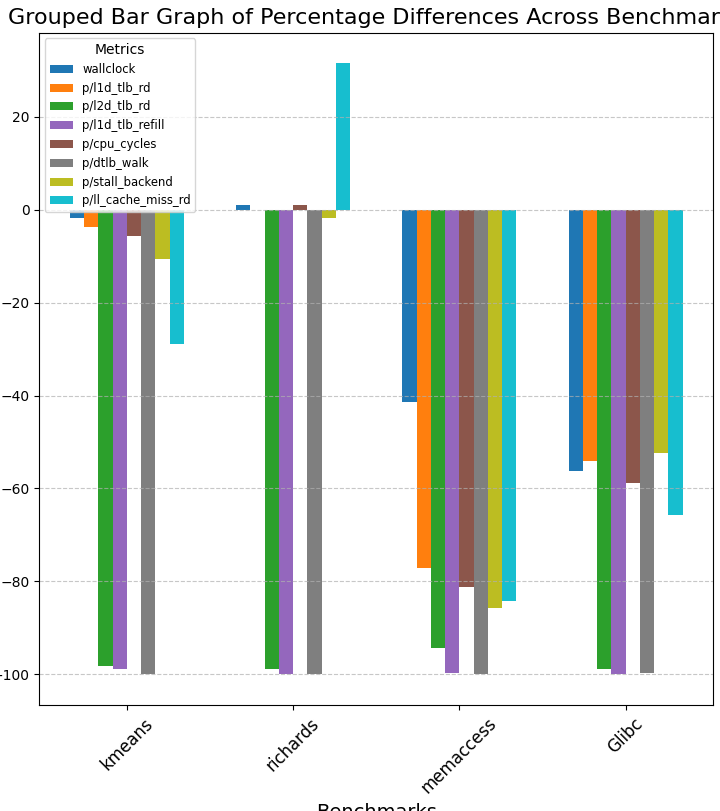
\includegraphics[width=.9\linewidth]{./diagrams/allbenchmarks.png}
\end{center}


The graph above highlights the performance comparison between the modified memory allocator and 
Jemalloc, the default memory allocator. The FAT pointer memory allocator, specifically optimized 
for use with huge pages, demonstrates a clear advantage in scenarios where memory allocation 
patterns benefit from its design. The results align with expectations, showcasing the impact 
of its capability to handle memory more efficiently by leveraging huge pages.

A particularly striking observation is the significant reduction in data TLB walks, 
L2 data TLB reads, and TLB refills—consistently showing a 90\% decrease across all 
benchmarks compared to Jemalloc. This improvement is due to the modified allocator's 
use of a single huge page entry at the L1 TLB layer. By enabling most address translations 
to be resolved directly at the L1 TLB, the need to walk through the deeper TLB hierarchy is 
largely eliminated. This reduction in translation overhead is a key factor in the allocator's 
superior performance for certain types of workloads.

The micro benchmarks, which are crafted to emphasize memory read operations, highlight the 
allocator's strengths. These tests simulate frequent and intensive memory access patterns, 
where the reduction in TLB misses directly translates into measurable performance gains. 
On average, the FAT pointer allocator achieves a 50\% reduction in wall clock runtimes for 
these workloads, underscoring its ability to optimize high-throughput memory operations.

On the other hand, macro benchmarks, which represent larger and more complex real-world applications, 
exhibit minimal differences in wall clock runtimes when using the FAT pointer allocator. 
This outcome is expected, as macro benchmarks typically involve a broader range of operations 
beyond memory allocation, diluting the impact of the allocator's optimizations. Additionally, 
the benefits of huge pages may be less pronounced for these workloads, as they are often 
bottlenecked by factors such as computation or I/O rather than memory translation overhead.

\begin{center}
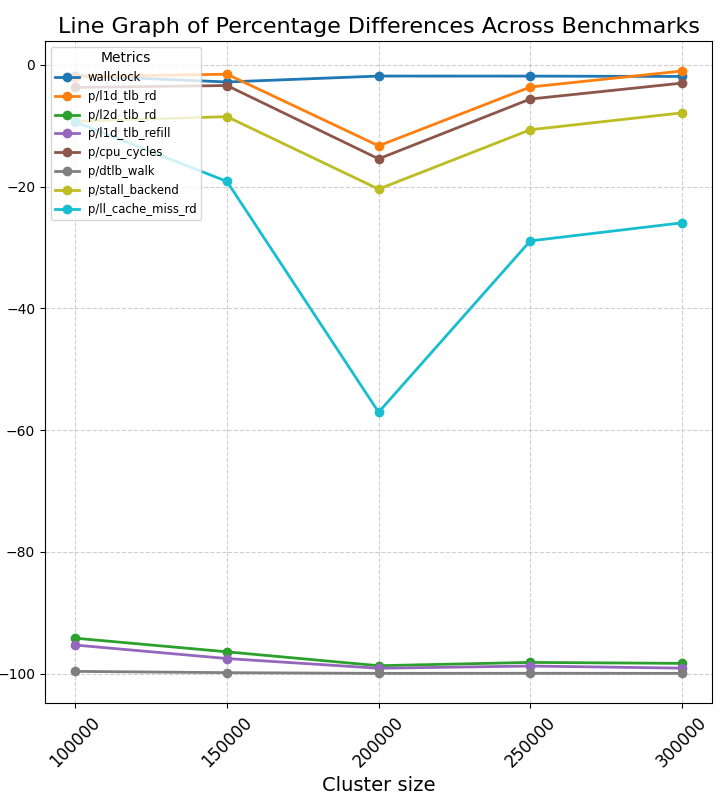
\includegraphics[width=.9\linewidth]{./diagrams/kmeans.png}
\end{center}

The K-means algorithm was executed with varying cluster sizes to evaluate the performance difference 
between the FAT pointer allocator and the baseline allocator as the workload scales. This analysis 
aimed to understand how the allocator's optimizations, particularly its ability to manage memory 
more efficiently with huge pages, impact performance under different workload conditions.

For most cluster sizes tested, the percentage difference in performance remained relatively 
consistent. This indicates that the allocator's efficiency scales predictably with increasing 
workload sizes, suggesting a stable and uniform benefit across different configurations. The 
consistent performance gain is likely due to the allocator's ability to minimize TLB misses 
and efficiently manage memory allocations for the centroid and data point structures used in 
the K-means algorithm.

However, an anomaly was observed at a cluster size of 2000, where the percentage difference 
deviated significantly from the trend. This irregularity could be attributed to several factors. 
At this cluster size, the memory access patterns and allocation behavior may align in a way that 
temporarily offsets the advantages of the FAT pointer allocator. For example, the memory layout 
might interact with system-level caching mechanisms or TLB behavior differently, leading to an 
unexpected change in performance. Additionally, the increased complexity of managing a higher 
number of clusters might introduce computational overhead that overshadows the memory allocator's 
optimizations.

This observation highlights the importance of testing across a range of workload sizes and 
configurations to uncover edge cases or specific scenarios where performance deviates from the 
expected pattern. Understanding these anomalies can provide insights into the allocator's 
behavior and guide future improvements to address such outliers. Despite the deviation at a 
cluster size of 2000, the overall results reaffirm the allocator's capability to maintain 
consistent performance benefits across most scenarios.
\subsection{Usability}
\label{sec:orgb4de289}
The FAT pointer memory allocator demonstrates significant potential for enhancing 
memory management in systems that benefit from huge page optimizations. Its design 
effectively reduces TLB misses, achieving up to 90\% fewer data TLB walks, L2 TLB reads, 
and TLB refills compared to Jemalloc. These improvements lead to noticeable performance 
gains, especially in micro benchmarks, where the allocator reduces wall clock runtimes 
by an average of 50\%.

The allocator integrates seamlessly into memory-intensive workloads, as evidenced by its 
consistent performance across varying cluster sizes in the K-means benchmark, with only 
minor anomalies observed under specific conditions. These outliers provide valuable 
insights into the allocator's interaction with system-level caching and memory translation mechanisms.

While the allocator excels in scenarios emphasizing high memory throughput, its impact on 
macro benchmarks is less pronounced. This suggests that its benefits are most relevant for 
applications with frequent and intensive memory operations rather than those constrained by 
computation or I/O bottlenecks.
\end{document}